%----------------------------------------------------------------------------------------
%	PACKAGES AND OTHER DOCUMENT CONFIGURATIONS
%----------------------------------------------------------------------------------------

\documentclass[twoside]{article}

\usepackage[sc]{mathpazo} % Use the Palatino font
\usepackage[T1]{fontenc} % Use 8-bit encoding that has 256 glyphs
\linespread{1.05} % Line spacing - Palatino needs more space between lines
\usepackage{microtype} % Slightly tweak font spacing for aesthetics

\usepackage[english]{babel} % Language hyphenation and typographical rules

\usepackage[hmarginratio=1:1,top=32mm,columnsep=20pt]{geometry} % Document margins
\usepackage[hang, small,labelfont=bf,up,textfont=it,up]{caption} % Custom captions under/above floats in tables or figures
\usepackage{booktabs} % Horizontal rules in tables

\usepackage{lettrine} % The lettrine is the first enlarged letter at the beginning of the text

\usepackage{enumitem} % Customized lists
\setlist[itemize]{noitemsep} % Make itemize lists more compact

\usepackage{titlesec} % Allows customization of titles
\renewcommand\thesection{\Roman{section}} % Roman numerals for the sections
\renewcommand\thesubsection{\roman{subsection}} % roman numerals for subsections
\titleformat{\section}[block]{\large\scshape\centering}{\thesection.}{1em}{} % Change the look of the section titles
\titleformat{\subsection}[block]{\large}{\thesubsection.}{1em}{} % Change the look of the section titles

\usepackage{fancyhdr} % Headers and footers
\pagestyle{fancy} % All pages have headers and footers
\fancyhead{} % Blank out the default header
\fancyfoot{} % Blank out the default footer
\fancyhead[C]{Search for Exoplanets $\bullet$ April 2018} % Custom header text
\fancyfoot[RO,LE]{\thepage} % Custom footer text

\usepackage{titling} % Customizing the title section

\usepackage{hyperref} % For hyperlinks in the PDF

\usepackage{multicol}
\usepackage{graphicx}
\graphicspath{{img/}}
\usepackage{float}

\newcommand{\code}[1]{\texttt{#1}}

%----------------------------------------------------------------------------------------
%	TITLE SECTION
%----------------------------------------------------------------------------------------

\setlength{\droptitle}{-4\baselineskip} % Move the title up

\pretitle{\begin{center}\Huge\bfseries} % Article title formatting
\posttitle{\end{center}} % Article title closing formatting
\title{Search for Exoplanets} % Article title

\author{%
\textsc{Petra Br\v{c}i\'c}\\% \\[1ex] 
\normalsize Applied Mathematics \\
\normalsize \href{mailto:petrabrcic94@gmail.com}{petrabrcic94@gmail.com} 
\and
\textsc{Sandro Lovni\v{c}ki}\\% \\[1ex] 
\normalsize Computer Science \\ 
\normalsize \href{mailto:lovnicki.sandro@gmail.com}{lovnicki.sandro@gmail.com}
}

\date{\today} 
\renewcommand{\maketitlehookd}{%
\noindent \textbf{\\Abstract:}
With the launch of Kepler space observatory in March 2009, the search for exoplanets has extensively began. There are currently $3,758$ confirmed exoplanets and contrary to the early approaches of validating exoplanet candidates by hand, machine learning has begun taking its toll on the subject. We would like to investigate neural network model for detecting transiting exoplanets from Kepler observatory light-curve data collected over a period of $4$ years, with over $200,000$ documented stars in our galaxy, the Milky Way. On April 18, 2018, a new satellite (TESS) has been launched, specificaly designed to search for exoplanets using the transit method. After it's 2-year planned mission, complete data should be available to public and more than $20,000$ new exoplanets are expected to be found.
\\\\
\textbf{Keywords:} Kepler, light-curve, exoplanet, machine learning, neural network, TESS.
}


%----------------------------------------------------------------------------------------

\begin{document}

% Print the title and table of contents
\maketitle
\tableofcontents
\newpage

%----------------------------------------------------------------------------------------
%	ARTICLE CONTENTS
%----------------------------------------------------------------------------------------
\begin{multicols}{2}

\section{Introduction}
In March 2009, NASA launched Kepler space observatory to discover Earth-size planets orbiting other stars in our galaxy. With most of the discoveries made after Kepler data was anounced, there are currently $3,758$ confirmed exoplanets in $2,808$ systems, with $627$ systems having more than one planet. Contrary to the early approaches of validating exoplanet candidates by hand or with humanly constructed models, recent years have been fruitfull for usage of machine learning for classifing Kepler's data.

\section{Methods}
There are many methods for detecting an exoplanet existance, as it can be seen in \cite{exo:methods}.\\
For example, \textit{gravitational lensing} method exploits the stars' gravitational fields' effect on magnification of distant background stars' light. If the star in question has a planet, its gravitational field makes a detectable contribution to the lensing effect. Over the past 10 years, just a $1000$ such events have been observed because specific alignment of bodies is required. Nonetheless, 19 exoplanets have been discovered using this method, whose full list is given in \cite{microlensing:exos}.\\
It is notable to mention \textit{radial velocity} method which uses variations in the speed with which specific star moves away or towards the Earth. Those variations are influenced by orbiting planet's gravitational pull and therefore we can also deduce the planet's mass. Up to 2012, this method was most effective for exoplanet detection whose full list is given in \cite{radial:exos}.

The most effective method today is the \textit{transit photometry}. When a planet crosses (transits) in front of its star, the star's brightness diminishes depending on planet relative size to it. To detect those brightness variations, observer's relative position must be properly aligned with star-planet axis which is not something one can control. The probability of a random alignment producing a transit in a system with Sun-sized star and a planet at 1AU \footnote{1 Astronomical unit $\approx$ Earth's ditstance to the Sun $\approx$ 150 million kilometres} from it is $0.47\%$. Ilustration of how those brightness variations are manifested in Kepler's data can be seen in Figure \ref{fig:kepler_curves}.
\begin{figure}[H]
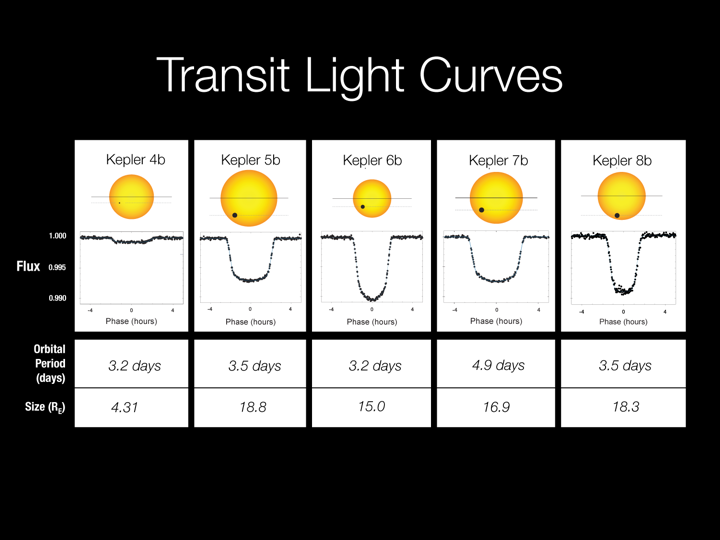
\includegraphics[width=0.5\textwidth]{KeplerLightCurves}
\caption{Illustration from \href{https://www.nasa.gov/mission_pages/kepler/main/index.html?FuseAction=ShowNews&NewsID=16}{Bill Borucki's Jan 2010 AAS Presentation}}
\label{fig:kepler_curves}
\end{figure}
\noindent Another disadvantage of this method is a high rate of false positives due to measurement precission and external noise that can be interpreted as a transit. For this reason, transit photometry is often combined with radial velocity to produce better results and eliminate false positives. The main advantage of transit photometry is planet's size deduction from light curve drops, which combined with transit photometry's mass deduction yields planet's density - a property much appriciated in search of habitable worlds. Also, by observing spectrum of light passed through the planet's atmosphere, one can detect which chemical elements are present. By April 12, 2018, Kepler detected $2,343$ exoplanets using transit photometry as a base method.



%------------------------------------------------
\section{Data}
Data used for this project is obtained by combining NASA Exoplanet Archive data for Threshold-Crossing Events which (currently) consists of $34032$ documented TCEs, each having $-CHECKNUMBER-$ column features and raw Kepler light-curves (star's flux (brightness) over time) at Mikulski Archive for Space Telescopes consisting of over $2000000 -CHECKNUMBER-$ star lightcurves monitored by Kepler.

Most important TCE features for our projects are \code{kepid}, \code{tce\_period}, \code{tce\_time0bk}, \code{tce\_duration} and \code{av\_training\_set} which (respectively) correspond to the Kepler identifier of host star, period of the event, time of the first appearance (more precisely; time of the begining of drop $+$ \code{tce\_duration}$/2$), duration of the event (drop in star's brightness) and label from set $\{PC,NTP,AFP,UNK\}$ meaning planet candidate, non-transit phenomena, astrophisical false positive and unknown. Those features will enable as to download just the Kepler light-curves of interest and later on to process each light-curve to extract and amplify features of TCE.

\subsection{Creating Dataset}
At the time of collecting our data, an older version of a TCE table was available with around $20000 --GETCORRECT-$ labeled TCEs. Distribution of \code{av\_training\_set} labels is as follows:
\begin{itemize}
	\item -NUMBER- TCEs with label PC (planet candidate)
    \item -NUMBER- TCEs with label NTP (non-transit phenomena)
    \item -NUMBER- TCEs with label AFP (astrophisical false positive)
    \item -NUMBER- TCEs with label UNK (unknown)
\end{itemize}
We used that table, specifically \code{kepid} colum to download just the light-curves for those stars from Kepler data. These light-curves are taking about $90$GB of space and are just a fraction of all the Kepler data.

Still, our machines are not fully prepared to tackle the preprocessing and learning from such a vast amount of not at all simple data, so we decided to choose randomly just some of the TCEs from table. We ended up selecting $1058$ TCEs labeled as planet candidate, $471$ TCEs labeled as astrophisical false positive and $734$ TCEs labeled as non transit phenomena.

As an example, here is a small table of selected features of one TCE documented for a star with \code{kepid} $9517393$:
\begin{center}
  \begin{tabular}{||c | c||} 
    \hline
    kepid & 9517393 \\
    \hline
    tce\_period & 219.322 \\
    \hline
    tce\_time0bk & 320.728 \\
    \hline
    tce\_duration & 0.5125000000000001 \\
    \hline
    av\_training\_set & PC \\
    \hline
    \ldots & \ldots \\
    \hline
    tce\_plnt\_num & 1 \\
    \hline
    tce\_eqt & 313.0 \\
    \hline
    \ldots & \ldots
  \end{tabular}
\end{center}

\subsection{Preprocessing Lightcurves}
In order to feed our model, we first need to process the raw light-curve into more useful and compact form. Raw light-curve is loaded as an array of smaller arrays called quarters which represent distinct periods in Kelper telescope's configuration, position, etc. We thus might expect quarters to be on a slightly different scale. In figure~\ref{fig:raw_lc} we show lightcurve for \code{kepid} $9517393$ right after loading \code{time} and \code{flux} arrays.
\begin{figure}[H]
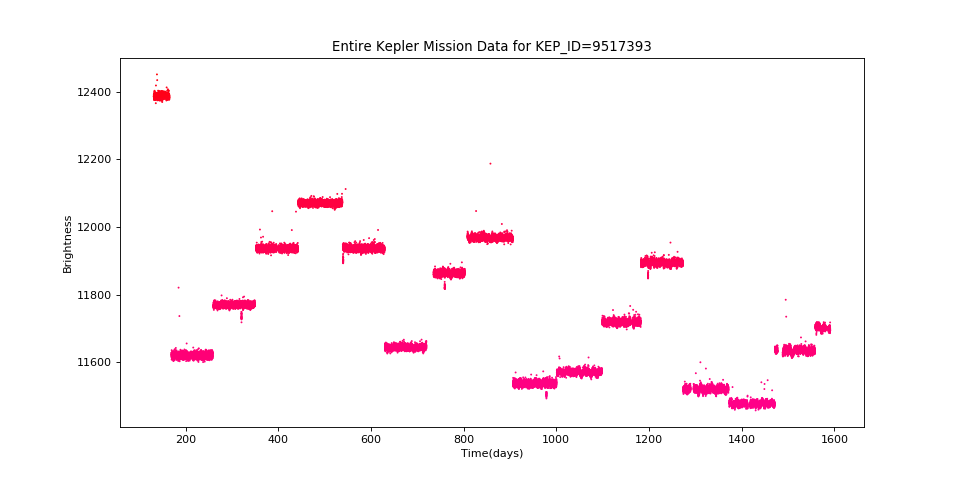
\includegraphics[width=0.5\textwidth]{rawLC-9517393}
\caption{Raw light-curve data}
\label{fig:raw_lc}
\end{figure}

It is easy to see that almost every star has an unpredictable variation in its flux, so the data is pretty distorted and irregular which is something that is to be avoided because it would interfere with our model's conclusions and feature extraction. Thus, we calculate a B-spline over the entire light-curve data, ignoring points that cannot be fitted or are of type \code{None}. This spline can be seen in figure!\ref{fig:raw_spline_lc} colored black.
\begin{figure}[H]
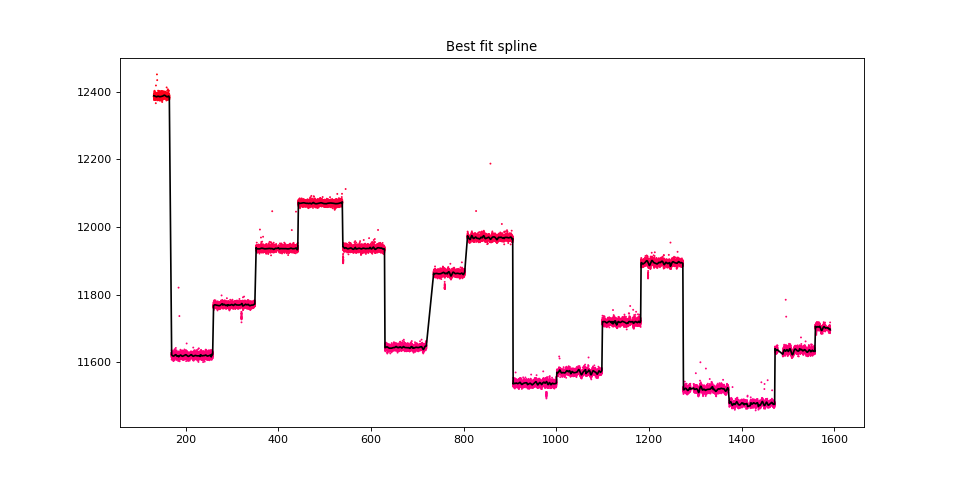
\includegraphics[width=0.5\textwidth]{splineLC-9517393}
\caption{Raw light-curve data with fitted B-spline}
\label{fig:raw_spline_lc}
\end{figure}

Next, we divide light-curve by the spline to obtain~\ref{fig:divided_lc}. Notice how specific TCEs can now be seen without even enlarging. 
\begin{figure}[H]
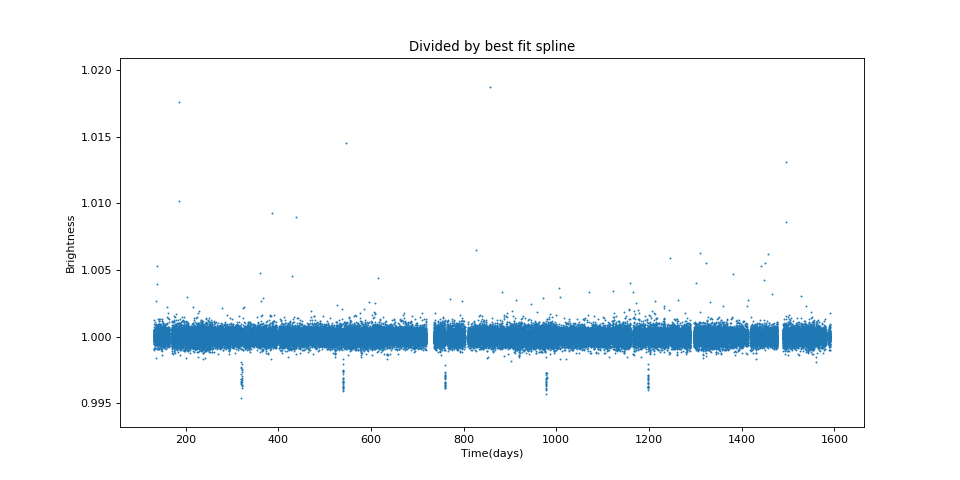
\includegraphics[width=0.5\textwidth]{divsplineLC-9517393}
\caption{Raw light-curve data divided by spline}
\label{fig:divided_lc}
\end{figure}

Now we need to exactly find the position of desired TCE which we know from TCE table, column \code{tce\_time0bk}. Focusing just on that segment of this plot, we get figure~\ref{fig:enlarged_tce}
\begin{figure}[H]
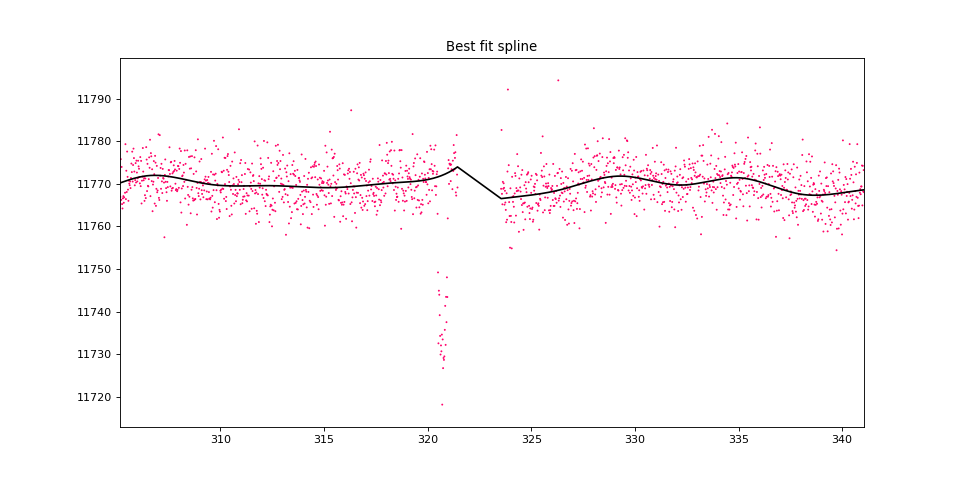
\includegraphics[width=0.5\textwidth]{splinezoomLC-9517393}
\caption{Enlarged area of the TCE}
\label{fig:enlarged_tce}
\end{figure}

We see that the amount of useful data of this "drop" is very poor, but we must remember that those events are periodic by definition so we hope that there is more instances of that same "planet" crossing during the lifetime of Kepler. We find the \code{tce\_period} from TCE table and fold every drop separated by \code{tce\_period} to \code{time0bk}. Now we divide TCE's duration into $201$ discrete points and calculate median value for flux in each of $200$ intervals in between. This results in a much richer, and uniform for all events, representation of a TCE which can be seen in!\ref{fig:folded_tce}. We call that view a "local view" and it is going to be the input of our model.
\begin{figure}[H]
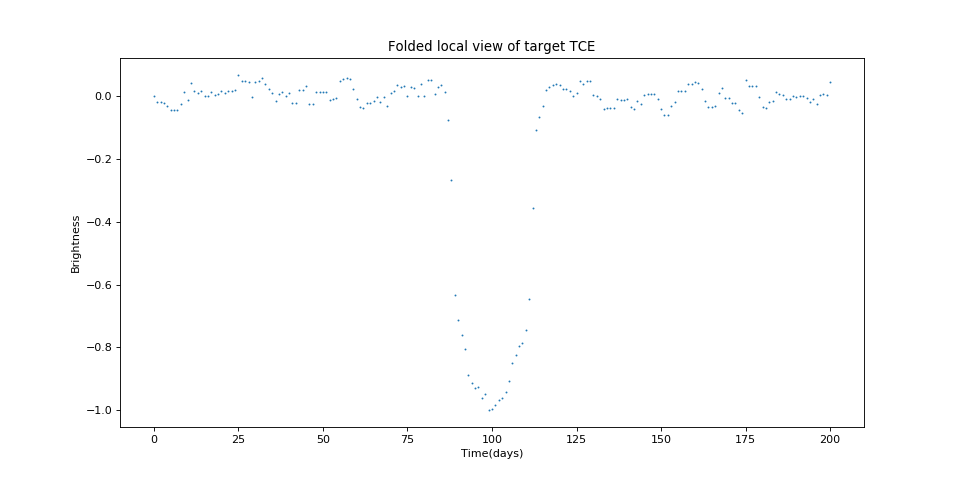
\includegraphics[width=0.5\textwidth]{localvierLCdrop-9517393}
\caption{Folded local view of the TCE}
\label{fig:folded_tce}
\end{figure}

%------------------------------------------------
\section{Convolutional Neural Network}


\subsection{1D Convolution}

\subsection{ReLu}

\subsection{Pooling}



%-----------------------------------------------
\section{Training}

\subsection{Parameters}

\subsection{Progress}


%----------------------------------------------
\section{Results}


%----------------------------------------------------------------------------------------
%	REFERENCE LIST
%----------------------------------------------------------------------------------------

\begin{thebibliography}{99}

\bibitem[1]{kepler:wiki}
\url{https://en.wikipedia.org/wiki/Kepler_(spacecraft)}

\bibitem[2]{tess:wiki}
\url{https://en.wikipedia.org/wiki/Transiting_Exoplanet_Survey_Satellite}

\bibitem[TESS]{tess}
\url{https://tess.mit.edu/}

\bibitem[3]{exo:methods}
\url{https://en.wikipedia.org/wiki/Methods_of_detecting_exoplanets}

\bibitem[4]{microlensing:exos}
\url{https://en.wikipedia.org/wiki/List_of_exoplanets_detected_by_microlensing}

\bibitem[5]{radial:exos}
\url{https://en.wikipedia.org/wiki/List_of_exoplanets_detected_by_radial_velocity}

\bibitem[6]{kepler:exos}
\url{https://en.wikipedia.org/wiki/List_of_exoplanets_discovered_using_the_Kepler_spacecraft}

\bibitem[Shallue and Vanderburg, 2017]{Shallue:2017}
Christopher J. Shallue, Andrew Vanderburg (2017).
\newblock Identifying Exoplanets with Deep Learning: A Five Planet Resonant Chain around Kepler-80 and an Eighth Planet around Kepler-90
\newblock arXiv:1712.05044 [astro-ph.EP]

\bibitem[Mikulski Archive for Space Telescopes]{mikulski}
\url{https://archive.stsci.edu/}

\bibitem[NASA Exoplanet Archive]{NASA:exos}
\url{https://exoplanetarchive.ipac.caltech.edu/cgi-bin/TblView/nph-tblView?app=ExoTbls&config=q1_q17_dr24_tce}

\bibitem[TCEs table]{tces}
\url{https://exoplanetarchive.ipac.caltech.edu/cgi-bin/TblView/nph-tblView?app=ExoTbls&config=q1_q17_dr24_tce}
 
\end{thebibliography}

%----------------------------------------------------------------------------------------

\end{multicols}{2}
\end{document}

